\section{Analysis applications and services} \label{sec:apps}

TOKIO connectors and tools interfaces are simply mechanisms to access I/O telemetry from throughout an HPC center.
As illustrated in Figure \ref{fig:portability-flow}, a higher-level analysis application was required to actually connect pytokio's interfaces to meaningful insight to an end-user.
That said, pytokio includes a number of example analysis applications and services that broadly fall into three categories.

\subsection{Command-line interfaces to pytokio} \label{sec:apps/cli}

Many connectors and tools present methods and functions that are valuable for users as-is.
For example, being able to retrieve application-level I/O performance telemetry with a single job id (as was presented in Section \ref{sec:architecture/tools} is an intrinsically useful operation.
To expose such useful functions directly to users without requiring that they write python, pytokio includes a set of command-line tools that simply convert command-line options into input arguments, pass these arguments to a single pytokio function, and then return the resulting output as ASCII to stdout.

Perhaps the most immediately valuable tools of this category are the command-line interfaces for each connector's serialization method, which allow specific component-level data to be quickly serialized into a generic and portable form.
For example, the LMT connector allows the contents of the LMT MySQL database to be serialized to a local SQLite file.
By serializing this data during a time period of interest to a portable format such as SQLite, the LMT data can be analyzed long after the LMT database itself has expired the data.
Furthermore, because the data is serialized to a standard and portable format, the SQLite database file itself could be shared and analyzed on remote systems for purposes of collaboration or reproducibility.

\subsection{Statistical analysis tools} \label{sec:apps/analysis}

\begin{figure}[t]
    \centering
    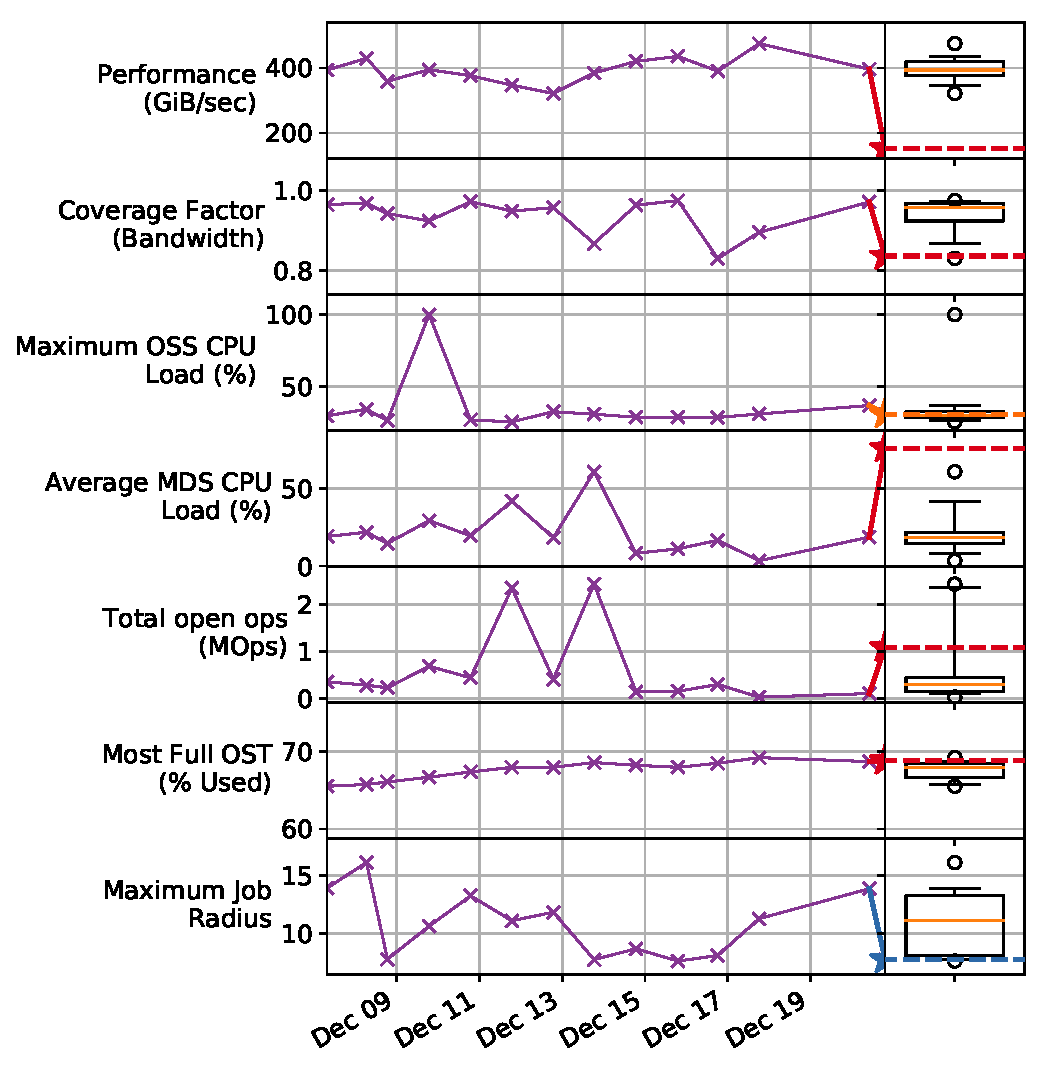
\includegraphics[width=1.0\columnwidth]{umami}
    \vspace{-.3in}
    \caption{UMAMI diagram of a simulated science campaign of HACC~\cite{Habib2012} simulations performed on NERSC's Cori system.  
    "Coverage Factor (Bandwidth)" is the fraction of global file system traffic originating from each HACC job, "Maximum Job Radius" represents the overall spread of each job's allocated nodes across the dragonfly network, and the remaining metrics represent server-side Lustre loads.}
    \label{fig:umami}
    \vspace{-.2in}
\end{figure}

pytokio arose from a proof-of-concept study that presented the concept of Unified Monitoring and Metrics Interface (UMAMI) diagrams~\cite{Lockwood2017}, and the tools required for a user to generate these diagrams is included in pytokio.
Figure \ref{fig:umami} is an example of such an UMAMI diagram for a case where poor performance on December 20 coincided with significant server-side bandwidth contention and metadata contention.
This diagram includes data obtained through many pytokio connectors: Darshan (Performance), LMT (Maximum OSS CPU Load, Average MDS CPU Load, Total Metadata Ops), Lustre health (Most Full OST), the Cray Service Database, and Slurm (both required to calculate the Maximum Job Radius).

To simplify the process of gathering data from all of these disparate sources of telemetry, pytokio includes the \texttt{summarize\_job} command-line tool provides a single command-line interface into every connector available.
When given either a list of job ids or a list of paths to Darshan log files (which contain job ids), \texttt{summarize\_job} infers the job start and end times, and then uses this data to retrieve the relevant Lustre system traffic and health data for the times during which each job ran.
It also retrieves the list of nodes that the job used via the Slurm connector and calculates several metrics representing the job's topology when mapped to the dragonfly network.
All of this data is then flattened into a set of key-value pairs all describing the specified job id and returned to the user in CSV format\footnote{This tool, as with many other pytokio components, uses pandas DataFrames internally to represent tabular data.  As such, pytokio can easily output to other supported formats such as JSON.}.
Each row of this CSV corresponds to a single job, and its columns are each a different metric produced by summarizing the output of one connector.

The CSV output of \texttt{summarize\_job} is then used to generate the UMAMI diagram itself.
The UMAMI diagram shown in Figure \ref{fig:umami} was generated using a Jupyter notebook, \texttt{tokio.analysis.umami.ipynb}, which included in the pytokio repository.
This notebook does the following:

\begin{enumerate}[leftmargin=*]
\item Loads the CSV file using \texttt{pandas.read\_csv()}
\item Performs basic filtering to discard job records which do not correspond to the analysis of interest (e.g., if a single job id generated multiple Darshan logs, but only one corresponds to the full-scale simulation execution).  Each job record corresponds to a row in the original \texttt{summarize\_job} output CSV.
\item Builds a set of \texttt{UmamiMetric} objects, each essentially representing a vector of measurements of one metric over time.  Each metric corresponds to a column in the original \texttt{summarize\_job} output CSV.
\item Creates a single \texttt{Umami} object (essentially an ordered dictionary) and appends each \texttt{UmamiMetric} object
\item Generates the UMAMI diagram using \texttt{UmamiMetric.plot()}
\end{enumerate}


okio's OST load visualizer which revealed that poor stage-out performance from DataWarp to Lustre (which occurs outside the purview of user applications) resulted from poor Lustre striping.  By using pytokio's connector abstractions, both of these analyses were implemented in only several dozen lines of code.

\begin{figure}[t]
    \centering
    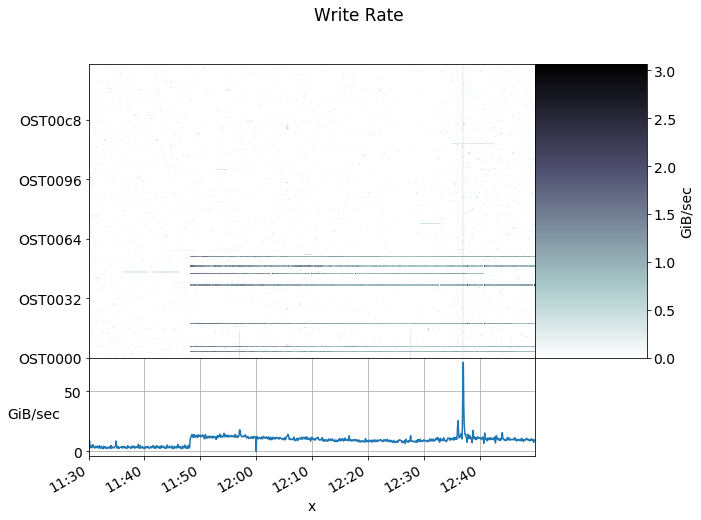
\includegraphics[width=1.0\columnwidth]{lustre-stageout-performance}
    \vspace{-.3in}
    \caption{Write rates of a stage-out operation from DataWarp to Lustre on Cori.  Each horizontal line represents a single OST performing intense I/O and whitespace is OST inactivity.  This visualization prompted the user to manually pre-stripe the DataWarp stage-out destination directory to ensure that the performance of all OSTs was available for subsequent stage-outs.}
    \label{fig:lustre-heatmap}
    \vspace{-.2in}
\end{figure}

\subsection{Data and analysis services} \label{sec:apps/services}